\SACCMD{contour}
\label{cmd:contour}

\SACTitle{概要}
利用内存中的数据绘制等值线图

\SACTitle{语法}
\begin{SACSTX}
CONT!OUR! [A!SPECT! ON|OFF]
\end{SACSTX}

\SACTitle{输入}
\begin{itemize}
\item ASPECT ON: 打开视图比开关。当这个开关打开时,等值线图的视口将会调整保持数据中y与x的比值
\item ASPECT OFF: 关闭视图比开关,这时将使用整个视口。
\end{itemize}

\SACTitle{缺省值}
\begin{SACDFT}
contour  aspect  off
\end{SACDFT}

\SACTitle{说明}
这个命令用于绘制二维数组数据的等值线图,包括SPECTROGRAM命令的输出。这个文件
操作的SAC文件必须``XYZ''类型的(SAC头段中IFTYPE为``IXYZ'')。有些命令可以
控制数据显示的方式:ZLEVELS控制等值线的数目以及间隔, ZLINES控制线型,
ZLABELS控制等值线标签,ZTICKS控制方向标记,ZCOLORS控制线条颜色。根据
contour选项的不同,有两种不同的绘制等值线算法。一种快速扫描方法用于既不
选择实线型也没有时标和标识的情况。另一种慢一点的方法,在绘图之前要组合
全部的线段。你可以使用快速扫描方法粗看你的数据,然后选择其他选项绘制最终
图形。

\SACTitle{例子}
下面的例子中,读入了XYZ文件contourdata,从头段中找出Z数据的范围。
选择等值线范围为700km到1150km,增量为25km。选择包括四种线型的线型表,其中第一个为实线。这个列表将每四条等值线重复一次。然后给等值线图起了个名字,最后绘制出来:
\begin{SACCode}
SAC> r ./contourdata 
SAC> lh iftype depmin depmax
  
  FILE: ./contourdata - 1
 -------------------
       IFTYPE = GENERAL XYZ (3-D) FILE
       DEPMIN = 6.977119e+02
       DEPMAX = 1.154419e+03
SAC> zlevels range 700 1150 increment 25
SAC> zlines list 1 2 3 4
SAC> title 'Katmai topography from survey data [inc = 25 km]'
SAC> contour
\end{SACCode}

\begin{figure}[H]
\centering
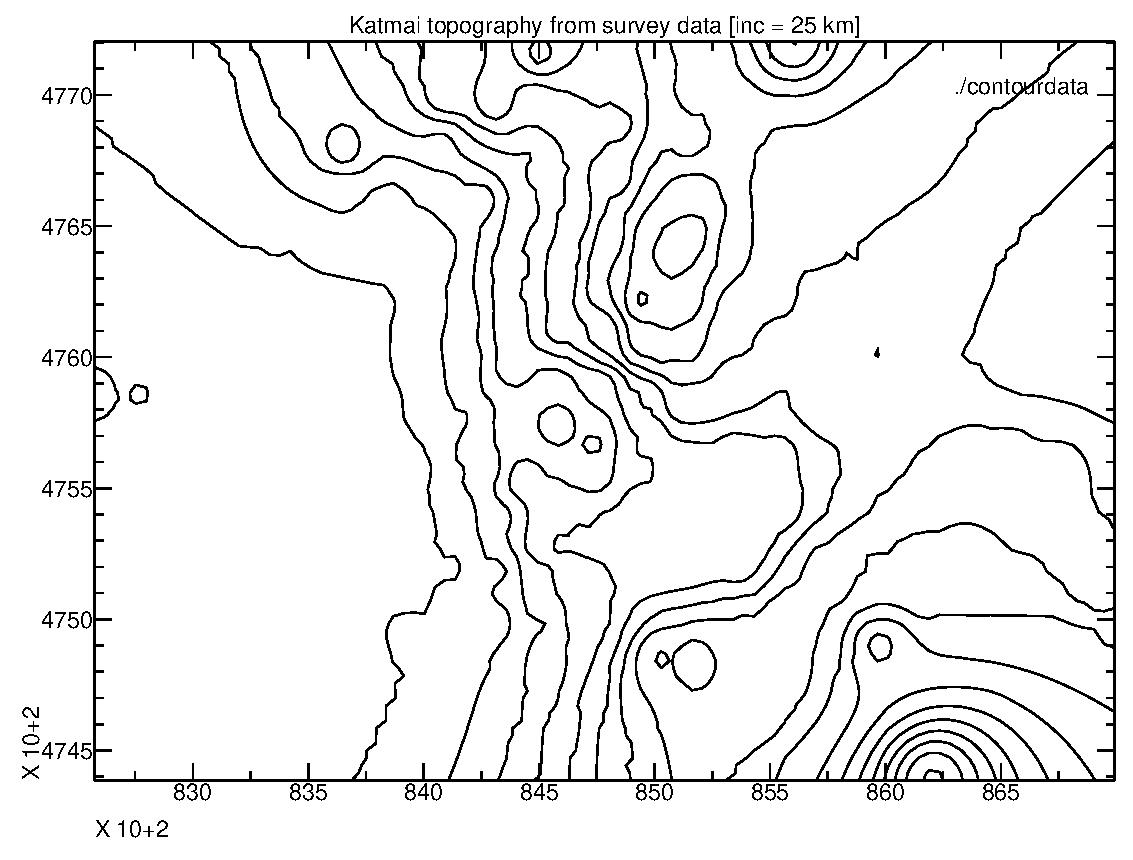
\includegraphics[width=0.9\textwidth]{contour1}
\caption{contour绘制等值线I}
\end{figure}

下面的例子中,使用同样的文件,但是显示选项不同。每四条等值线有一个整数标签。
每条等值线之间都有一个指向向下的箭头。所有等值线为实线型:
\begin{SACCode}
SAC> r ./contourdata 
SAC> zlevels range 700 1150 increment 25
SAC> zlabels on list int off off off
SAC> zticks on direction down
SAC> zlines list 1
SAC> title 'Katmai topography from survey data [labels and ticks]'
SAC> contour
\end{SACCode}

\begin{figure}[H]
\centering
\includegraphics[width=0.9\textwidth]{contour2}
\caption{contour绘制等值线图II}
\end{figure}

\SACTitle{头段变量改变}
要求: iftype (为``IXYZ''), nxsize, nysize

使用: xminimum, xmaximum, yminimum, ymaximum

\SACTitle{相关命令}
\nameref{cmd:zcolors}、\nameref{cmd:zlabels}、\nameref{cmd:zlevels}、
\nameref{cmd:zlines}、\nameref{cmd:zticks}、\nameref{cmd:spectrogram}
